\documentclass[usenames,dvipsnames]{standalone}
\usepackage{tikz}
\usepackage{tikz-network}
\usepackage{libertine}
\usepackage{libertinust1math}
\usepackage{pgfplots}

\usepackage[T1]{fontenc}
\usetikzlibrary{patterns.meta,decorations.pathmorphing}

\begin{document}
	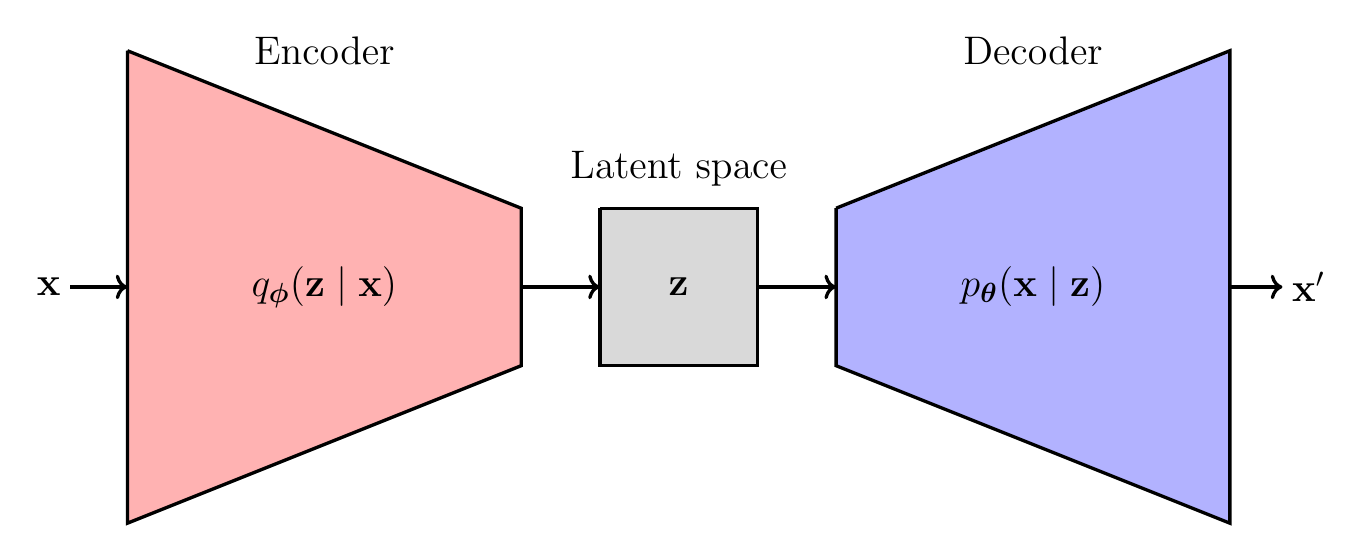
\begin{tikzpicture}
		
		% input into encoder
		\node[] (x) at (-1, 0) {\Large $\mathbf{x}$};
		\draw[->, very thick] (x) -- (0, 0);
				
		% encoder
		\draw[fill=red!30, very thick] (0, 3) -- (5, 1) -- (5, -1) -- (0, -3) -- (0, 3);
		\node[] (z) at (2.5, 0) {\Large $q_{\boldsymbol{\phi}}(\mathbf{z} \mid \mathbf{x})$};
		\node[] (z) at (2.5, 3) {\Large Encoder};
		\draw[->, very thick] (5, 0) -- (6, 0);
		
		% latent space
		\draw[fill=gray!30, very thick] (6, 1) -- (8, 1) -- (8, -1) -- (6, -1) -- (6, 1);
		\node[] (z) at (7, 0) {\Large $\mathbf{z}$};
		\node[] (z) at (7, 1.5) {\Large Latent space};
		\draw[->, very thick] (8, 0) -- (9, 0);

		% encoder
		\draw[fill=blue!30, very thick] (9, 1) -- (14, 3) -- (14, -3) -- (9, -1) -- (9, 1);
		\node[] (z) at (11.5, 0) {\Large $p_{\boldsymbol{\theta}}(\mathbf{x} \mid \mathbf{z})$};
		\node[] (z) at (11.5, 3) {\Large Decoder};
		
		% output from decoder
		\node[] (xp) at (15, 0) {\Large $\mathbf{x}^\prime$};
		\draw[->, very thick] (14, 0) -- (xp);
		
		
	\end{tikzpicture}
\end{document}